\documentclass[SE,lsstdraft,authoryear,toc]{lsstdoc}
% lsstdoc documentation: https://lsst-texmf.lsst.io/lsstdoc.html
\input{meta}

% Package imports go here.

% Local commands go here.

%If you want glossaries
%\input{aglossary.tex}
%\makeglossaries

\title{CCW/Rotator Synchronous Motion Limit Switch Characterization}

% Optional subtitle
% \setDocSubtitle{A subtitle}

\author{%
Austin Roberts, Andrew Heyer
}

\setDocRef{SITCOMTN-011}
\setDocUpstreamLocation{\url{https://github.com/lsst-sitcom/sitcomtn-011}}

\date{\vcsDate}

% Optional: name of the document's curator
% \setDocCurator{The Curator of this Document}

\setDocAbstract{%
The Camera Cable Wrap / Camera Rotator synchronous motion limit switch characterization will identify the optimal placement of the limit switches based on a variety of factors. In addition, this characterization will define a recommendation for follow on work to be conducted due to the design differences between the originally design bulkhead plate and the redesigned bulkhead plate which houses the limit switches.
}

% Change history defined here.
% Order: oldest first.
% Fields: VERSION, DATE, DESCRIPTION, OWNER NAME.
% See LPM-51 for version number policy.
\setDocChangeRecord{%
  \addtohist{1}{YYYY-MM-DD}{Unreleased.}{Austin Roberts}
}


\begin{document}

% Create the title page.
\maketitle
% Frequently for a technote we do not want a title page  uncomment this to remove the title page and changelog.
% use \mkshorttitle to remove the extra pages

% ADD CONTENT HERE
% You can also use the \input command to include several content files.

\section{Executive Summary}

The characterization of the limit switches that protect the utility
lines that run from the Camera Cable Wrap to the back of the Camera was
performed on the Tekniker designed bulkhead plate which connects to the
Camera Cable Wrap. This characterization was performed on the Camera
Cart on the 3\textsuperscript{rd} floor of the observatory without
ComCam or LSSTCam installed on the Camera Rotator. The primary goal of
the characterization was to determine the optimal placement of the limit
switches. Prior to completing the characterization it was brought to our
attention that the bulkhead plate had been redesigned by SLAC due to
complexities with the camera installation. At this stage of the
characterization, it has been determined that the limit switches should
be placed at +/- 3.5 deg from the center line. This was largely driven
by the distance required to release the limit switch without activating
the opposite limit switch. This could lead to a worst case scenario
which would lead to a 5.86 deg angular difference which is larger than
the requirement of 5 deg. Due to differences in the design of the SLAC
bulkhead plate and this characterization being performed without a
representative load and CG on the Rotator, this characterization will
need to be performed again on the SLAC bulkhead plate after ComCam is
installed on the Rotator and before the utilities are connected.
Depending on the results of the characterization of SLAC bulkhead plate
the worst case maximum angular difference may need to be addressed.

\section{Overview}

\subsection{System Overview}

The system being characterized is the Camera Cable Wrap (CCW), the
Camera Rotator, and the Wobble Assembly. The Wobble assembly connects to
the CCW via the bulkhead plate and to the ComCam/LSSTCam via the wobble
plate per LTS-156. The bulkhead plate has a limit switches mounted in
the positive and negative direction in relation to the 0 degree location
and a revolute joint with adjustable detection cams in the positive and
negative direction. These features are designed to protect the utility
lines from damage due to excessive twist between the CCW and the Camera.
See Figure 1 below. The bulkhead plate and the limit switches rotate
with the CCW and the wobble plate, central linkage rod, and the
detection cams rotate with the Camera. The Camera is rotated by the
Camera Rotator. Activating either the positive or negative limit switch
will generate a Safe Torque Off (STO) to the CCW Interlock System and
the Rotator Interlock System to remove power to the drives. Without
ComCam or LSSTCam the wobble assembly cannot be installed. In this
situation, a single central connecting rod was connected to a metallic
bar attached to the Camera Rotator's camera mounting ring. See Figure 2
below. The characterization was performed on the Camera Cart on the 3rd
floor of the observatory.

\begin{figure}
\begin{center}
  \includegraphics[width=6.5in,height=6.28472in]{media/Figure_1.png}
\end{center}
\caption{Bulkhead Plate with Temporary Central Rod}
\label{fig:Figure_1}
\end{figure}

\begin{figure}
\begin{center}
  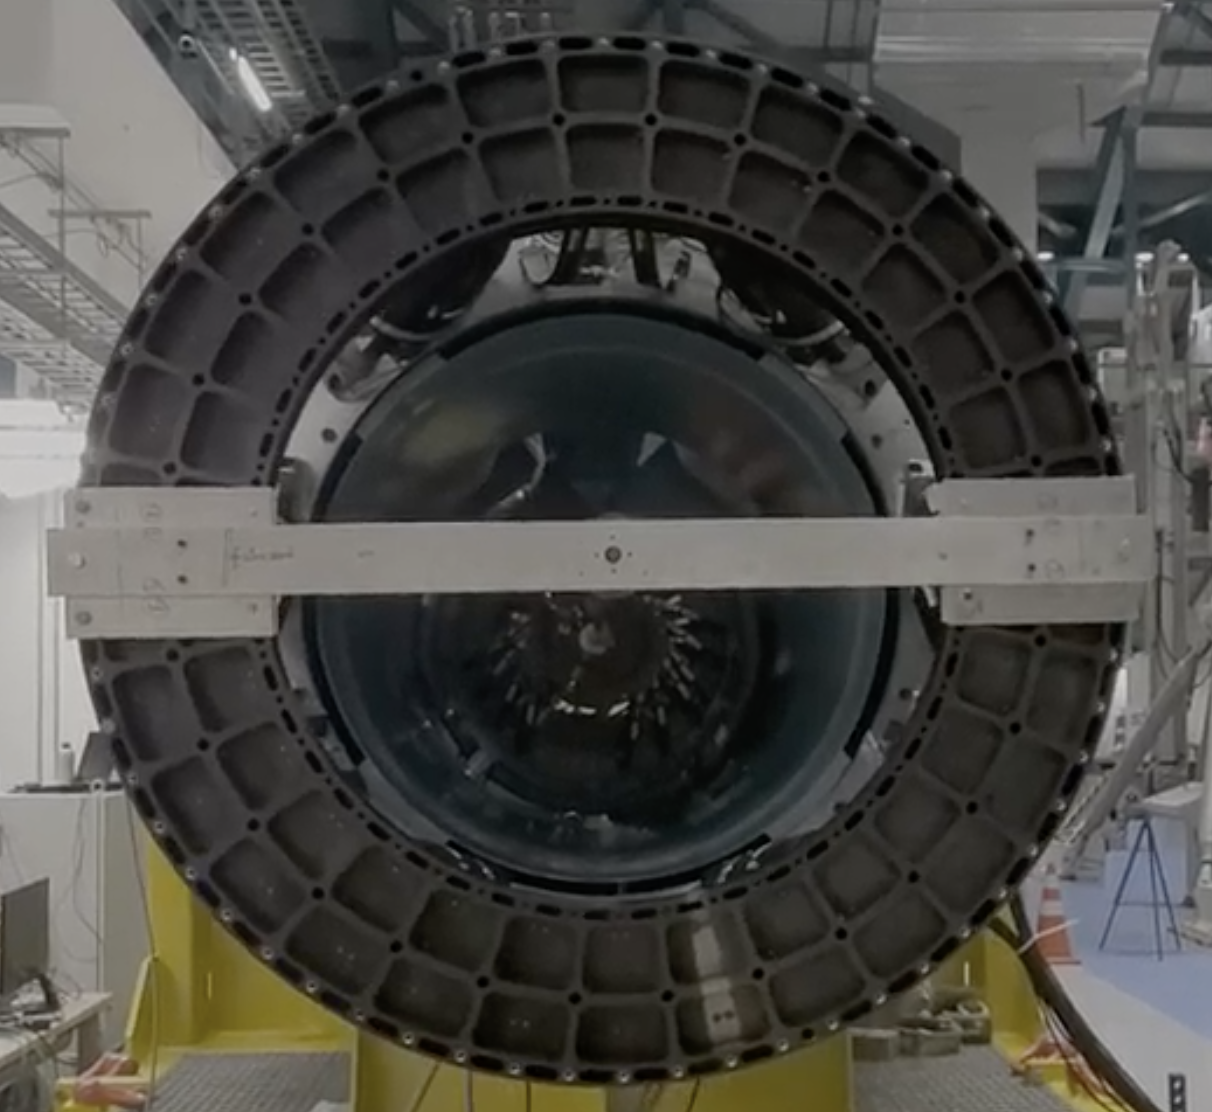
\includegraphics[width=6.5in,height=5.96389in]{media/Figure_2.png}
\end{center}
\caption{Camera Rotator Temporary Connection Bar}
\label{fig:Figure_2}
\end{figure}

\subsection{Objective}

The objective of this characterization is to find the allowable position
range of the positive and negative limit switches and provide a
recommendation of where they should be positioned. This requires finding
the exact position that the limit switches are currently activated,
finding the back off distance required to release the limit switches,
and finding the maximum distance for the CCW and Camera Rotator to come
to a complete stop after activating the limit switches.

\subsection{Requirements}

The following are the relevant requirements for the synchronous motion
between the CCW and the Camera Rotator.

\underline{LTS-103}

\begin{itemize}
\item
  3.10.13 MCS Camera Cable Wrap Positioning Command

  \begin{itemize}
  \item
    \textbf{Specification:} The camera cable wrap shall be slaved to the
    camera rotator.
  \end{itemize}
\end{itemize}

\underline{LTS-218}

\begin{itemize}
\item
  3.3.7 Rotation Drive Synchronization with Camera Rotator

  \begin{itemize}
  \item
    \textbf{Specification:} During slewing and tracking, the camera
    cable wrap rotation shall remain synchronized with the camera
    rotator to better than 2.2 degrees. An absolute rotation sensing
    encoder shall be incorporated on the rotation drive unit to provide
    position feedback to the telescope control system (TCS).
  \end{itemize}
\item
  3.3.8.1 Slewing Velocity Range

  \begin{itemize}
  \item
    \textbf{Specification:} The rotation drive unit shall be able to
    reach any velocity between 0 and 3.5deg/sec with a goal of
    5.25deg/sec in both rotation directions.
  \end{itemize}
\item
  3.16 Safety Pull Cord

  \begin{itemize}
  \item
    \textbf{Specification}: The functionality of the safety pull-cord
    has been replaced by limit switches now specified in LTS-156.
  \end{itemize}
\item
  3.3.1 Rotation Range

  \begin{itemize}
  \item
    Specification: The camera cable wrap shall be designed to rotate
    over a 180 degree operational range (+/- 90 degrees either side of
    centered position). This 180 degree range must be achievable without
    exceeding any software limit, limit switch or hard stop,
    consequently, an additional 8 degrees (+/-4) is required to
    accommodate these items. The software limits shall limit the motion
    to the 180 degree range. The limit switches shall stop the motion
    within 2 degrees of meeting this maximum operational range. The hard
    stops shall stop the motion within another 2 degrees of the limit
    switches.
  \end{itemize}
\end{itemize}

\underline{LTS-156}

\begin{itemize}
\item
  The limits shall be adjusted to nominally stop rotation for any twist
  between the bulkhead plate and the wobble plate greater than +/- 3.5
  degrees with adjustment range from 2.5 degrees to 5 degrees.
\item
  The limit switch shall be tested over the range of travel of the
  wobble plate as specified below.

  \begin{itemize}
  \item
    The wobble plate radial motion is +/- 110mm.
  \item
    The wobble plate tilt about its center is +/- 3 degrees.
  \item
    The wobble plate Z motion is +/- 15mm.
  \end{itemize}
\end{itemize}

\underline{LTS-206}

\begin{itemize}
\item
  3.4.5.1 Rotator Slewing Velocity Range

  \begin{itemize}
  \item
    \textbf{Specification:} During a rotator slew, the Camera Rotator
    shall be able to reach any velocity between 0 and 3.5deg/sec with a
    goal of 5.25deg/sec in both rotation directions.
  \end{itemize}
\item
  3.4.4 Rotator Rotation Range

  \begin{itemize}
  \item
    \textbf{Specification:} The Camera Rotator shall be designed to
    rotate over a 180 degree operational range (+/-90 degrees TBR). This
    range must be achievable without reaching any software limit, limit
    switch or hard stop. The limit switches shall stop the motion within
    2 degrees of meeting this maximum operational range. The hard stops
    shall be within another 2 degrees of the limit switches.
  \end{itemize}
\end{itemize}

\underline{LSE-80}

\begin{itemize}
\item
  CA-TS-MEC-ICD-0058 Maximum Allowed Camera Motion at Bulkhead Plate

  \begin{itemize}
  \item
    \textbf{Specification:} The telescope shall ensure that the maximum
    transverse and axial motions of the back end of the camera utility
    trunk are no larger than \textbf{UTradialMotion} transverse,
    \textbf{UTaxialMotion} axial load, and \textbf{UTrotMotion} angular
    rotation around a radial line.
  \item
    UTrotMotion = 5 degrees
  \end{itemize}
\end{itemize}

\appendix
% Include all the relevant bib files.
% https://lsst-texmf.lsst.io/lsstdoc.html#bibliographies
\section{References} \label{sec:bib}
\renewcommand{\refname}{} % Suppress default Bibliography section
\bibliography{local,lsst,refs_ads,refs,books}

% Make sure lsst-texmf/bin/generateAcronyms.py is in your path
\section{Acronyms} \label{sec:acronyms}
\input{acronyms.tex}
% If you want glossary uncomment below -- comment out the two lines above
%\printglossaries





\end{document}
